
\subsection*{Modeling the naturalistic stimulus and verbal recall}
We fit a topic model \citep{BleiEtal03} to hand-annotated text descriptions of scenes from the video. The text descriptions contained details of the scene such as the characters present, location, and a short summary of the scene (see Fig.~\ref{fig:schematic} for example text). As depicted in Fig.~\ref{fig:model}A, the topic vectors are sparse and change slowly over time. Furthermore, there are clear transitions from one topic ``state'' to the next, possibly indexing scene transitions in the stimulus. To get a better handle on this temporal structure, we computed a timepoints (1976) by timepoints (1976) correlation matrix of the video model (Fig.~\ref{fig:model}C).  This correlation matrix reveals that the model has a strong, block-diagonal structure with very low off-diagonal correlation values, suggesting the representations of each block are unique and highly discriminable. We found that the ``narrative details'' (a few sentences summarizing the dialogue and specific happenings of the scene) of the video were the most important feature driving this model structure (see Fig.~\featureimportance A).

After watching the video, participants verbally recalled (in order) as much of the episode as they could.  We used the same topic model (fit with the text descriptions of the video) to transform participants' verbal recall transcripts. An example participant's (\#13) recall model is plotted in Fig.~\ref{fig:model}B. Notably, participant \#13's recall model appears visually similar to the video model. Similar to the video model analysis (Fig.~\featureimportance A), we found that the ``narrative details'' feature was most important for driving the video/recall relationship (Fig.~\featureimportance B).  Like the video model, topic vectors were sparse and changed gradually.  Then, we investigated the temporal structure of the recall matrices. From each participant's recall model, we computed a sentences (68 to 294) by sentences (68 to 294) correlation matrix (Fig.~\ref{fig:model}D). Like the video model, each participant's recall correlation matrix exhibited a strong block-diagonal structure (Fig.~\corrmats). Notably, this suggests that participants recounted the video in discriminable segments, likely related to the recall of specific events from the video.




\subsection*{Segmenting the video and recall models into ``events''}
As described above, a striking feature of both the video and recall correlation matrices is a strong, block structure along the diagonal of the matrices (see Fig.~\ref{fig:model}C,D).  We hypothesized that this structure might arise from transient stability in the "theme" of both the video and of participants' memory for the video. We hypothesized that specific events described by a participant could be ``matched'' to specific video events by computing the similarity (i.e., correlation) between their topic vectors. In other words, the video event that is most thematically similar to a particular recall event is the event that the participant is most likely describing. To test this idea, we segmented the video and recall models in $k$ events (i.e., states) using a hidden Markov model ~\citep{BaldEtal17}. Our algorithm determined 34 events for the video model and a range of values (range: 8-27; mean: 15.41; SD: 5.6) for the recall models (see Methods for details on choosing an optimal $k$ value).  The events discovered for the video model and a representative participant's recall model are highlighted as yellow rectangles outlining blocks along the diagonal of the correlation matrices (Fig.~\ref{fig:model}C,D).

Next, we created a video ``event model'' by averaging together neighboring topic vectors that the were classified to be in the same event, resulting in an events (34) by topics (100) matrix (Fig.~\ref{fig:model}E).  We performed the same procedure for the recall matrices (Fig.~\ref{fig:model}F). Then, we computed the correlation between video and recall event models, resulting in a video events (34) by recall events (8-27, depending on the participant) correlation matrix (Fig~\ref{fig:model}G for example, Fig.~\matchmats for all participants). These matrices represent the similarity (correlation) between each video event and each recall event (for each participant). To determine which video event a particular recall event was most likely describing, we found the index of the video event with the highest correlation to the recall event (i.e., the argmax).  This is depicted in Fig.~\ref{fig:model}G as the cells highlighted with a yellow border. Notably, our algorithm suggests that the example participant recalled most of the video events and did so in order.

Then, we computed a group-averaged recall event model and video-recall event correlation matrix. For each participant (and each recall event), we sorted the recall event vectors (across all participants) according to the video event with the highest correlation. We then averaged the recall event vectors within each group. This yielded an average recall event vector for all but one (of 34) video events, since no participant remembered one of the events according to our model. Lastly, we computed an average recall event (34) by video event (34) correlation matrix, and highlighted the cell with the highest correlation value with a yellow border (Fig.~\ref{fig:model}H). Notably, this matrix displayed high correlation values along the diagonal and low correlations in the off-diagonal cells. This suggests that on average, participants were able to recapitulate the events in the episode in a specific, sequential and highly descriminable way.

\subsection*{The trajectory of a naturalistic experience is preserved in recall}
Classic approaches to studying free recall in episodic memory (such as overall accuracy and serial position curve) focus on the quantity of information recalled \citep{Murd62a}. More recent metrics (such as lag-CRP, semantic and temporal clustering) go further to describe list-level memory organization \citep{Kaha96, PolyEtal09}. However, these approaches cannot (and were not designed to) capture the rich temporal dynamics inherent in naturalistic stimuli and associated recall of those experiences. In the next set of analyses, we test the hypothesis that successful recall of a naturalistic stimulus entails recovering the trajectory of a stimulus.

%%%%



These features of real world memory provide a stark contrast with classic list-learning memory tasks that ask participants to reproduce from memory a set of studied items (e.g. words)-- whereby each word's meaning is distinct from surrounding words, and successful memory for a given word entails reproducing it exactly during recall.  So how might one go about assessing the quality of real world memory?  Which analysis methods and findings from the list-learning literature apply to real world learning?  And how might one go about formally characterizing whether (or how well) the ``gist'' of a memory has been accurately remembered?




A defining characteristic of 

One approach to studying memory for naturalistic experiences and real life events in the laboratory has been to quantify the participant's ability to recall specific aspects of the experience, such as the people, places, and things encountered~\citep[e.g.\ for review see][]{KoriGold94}.  This essentially 

Human memory studies typically assess memory for the elements within an experience, such as the people, places and things encountered. However, real life experiences can also be described in terms of their temporal structure (i.e., how the contents relate/change over time).  For instance, naturalistic experiences are autocorrelated in space and time on short timescales. In other words, the contents of an experience often change gradually and are therefore similar from moment to moment. As an example, many of us spend our mornings/evenings at home and much of our days at work (e.g., in an office). While the specific happenings within these contexts differ, they are often highly correlated (and thus predictable) within an experience. Furthermore, our experiences can also be characterized by longer timescale correlations. For example, consider returning to your office after taking a lunch break. The spatial contexts before and after lunch are highly similar, but separated in time. Thus, while evaluating the ability to recall the isolated elements of an experience has been a fruitful way to learn about human memory, another important dimension to consider is the temporal structure of the remembered experience, and how the temporal structure of the memory relates to the original experience. These recurrent and gradually changing temporal dynamics are not typically present in traditional memory studies, but are likely critical to understanding how our memory systems encode, store and retrieve our life experiences.



Another interesting feature of the recall matrices is the off-diagonal structure, which represents the use of language that generalizes to more than one event. To characterize this aspect of the recall structure, we averaged the rows of the recall matrices according to the k events computed in the analysis described above.  This reduced the recall matrices from \# of sentences to k rows. Then, we computed k by k correlation matrices, representing the similarity of each event to each other event. To visualize these recall `networks', we embedded the k by topics matrices into a 2-dimensional space using Multidimensional Scaling (MDS), where each dot represents an event and the color of the dot represents the event index.  Then, we connected each event with a line where the color and line weight was proportional to the strength of the correlation between the events. These network plots can be seen in Fig X. To hypothesized that stronger correlations between recall events would

\subsubsection{Temporally aligning the stimulus and recall}
While most participants were able to recall most of the scenes in order, the rate of verbal description varied by participant and timepoint (Supp Fig X). Because of this participant-dependent non-linear relationship between stimulus and recall time, averaging the video-recall correlation plots across participants attenuates the robust within-participant effects. While further exploration of individual differences in recall rates is interesting, our primary goal here was to develop a model capable of accurately characterizing the content recovered during recall and explore how that varied across participants.  To that end, we leveraged dynamic time warping (DTW, REF) to temporally align the stimulus and recall matrices.  The algorithm returns a path of indices that bring the two timeseries into maximal temporal alignment (within constraints, see Methods for details).  For each participant, we computed the path and then warped the video model and recall model according to it. The length of the warp path varied by participant, and so the length (number of timepoints) of the warped video/recall matrices also varied by participant (range: X-X). To account for these differences, we resampled the timeseries back to the length of the stimulus (1976 time samples).

\subsection{fMRI analyses}
Seventeen participants watched the first 50 minutes of Episode 1 of BBC's Sherlock. The video was split into two parts of approximately equal length (946 and 1030 TRs). All data were preprocessed and transformed to 3mm MNI space as described in the paper. Data were zscored across time at every voxel. 6mm smoothing was applied.
Files are cropped so that all video-viewing data are aligned across participants, and all recall data are aligned to the scene timestamps below. The cropping includes a constant 3-TR (4.5 sec) shift to correct for hemodynamic lag.

\subsubsection{Univariate subsequent memory analysis}
To characterize brain regions involved in memory encoding, we conducted an analysis inspired by prior studies investigating the  `subsequent memory effect' (Paller and Wagner).  For each participant, we computed the correlation between topic vectors at each timepoint of the video model and recall model (they were temporally aligned with DTW and resampled to 1976 timesamples). The result was a 1 x 1976 vector of correlation values representing how similar each moment of the video model was to each moment of the recall model. Then, to compute the average correlation, we Fisher's z transformed the correlation vectors, averaged them together, and then inverse Fisher's z transformed them.  Finally, we mean centered the vector.  This 1 x 1976 vector represents memorable/unmemorable parts of the video, and be thought of as a `continuous' extension of a subsequent memory regressor.  We convolved the timeseries with a double gamma function (PARAMS) to account for the hemodynamic response, and used it as a model for each voxel's activity timeseries (using FSL software).  Finally, to aggregate across participants, we performed a mixed effects (ordinary least squares) analysis, thresholding at p<.001 and cluster correcting a p<.05.

\subsubsection{Multivariate searchlight analyses}
Our multivariate analyses were designed to capture brain regions whose timepoint-by-timepoint correlational structure mirrors the correlational structure of the video and recall topic models during video viewing. To that end, we conducted a searchlight analysis (5x5x5 voxel cube) where for each cube, we correlated the model timepoint-by-timepoint correlation matrix with the neural correlation matrix. To aggregate across participants, we computed Fisher's z transformed the correlations and then averaged.  To assess significance, we recomputed this group analysis 100 times, but randomly phase shifted the model (by \# of timepoints - 1) by the same amount for each participant but different amounts for each permutation to build a null distribution of correlation values. Finally, we thresholded the group averaged correlation maps where the `real' correlation value for a given voxel exceeded the 95th percentile of the null distribution.

We first performed this analysis using the unwarped video model. Thus, the same model was applied to each participant and each searchlight cube. We then performed this analysis on the participant-wise recall models. To correct for non-linearities between the video model and recall models, for each participant we used DTW to temporally align the matrices. The algorithm recovers a path of coordinates that would bring the video and recall model in maximal temporal alignment. We used this path to warp the fMRI data and the recall model into alignment (separately for each participant). Then, we performed the exact same analysis as described above, using a searchlight to correlate the timepoint-by-timepoint recall and neural correlation matrices. The statistics for both analyses were computed as described above.

\subsubsection{Accounting for nonlinearities between video and recall models}
For many participants, the rate of recall changed over time (see Supp Fig X for an example). This becomes problematic if averaging the video/recall correlation matrices because the different recall rates distort the group average matrix. To correct for differences in recall rates across participants, we used dynamic time warping (DTW).  Briefly, DTW finds the path that maximizes the temporal alignment between two timeseries (REF). For each participant, we used DTW to temporally align the video model and the participant-specific recall model. Because the path is different for each participant, the length of the warped matrices varied across participants (range: X to X). To account for this, we resampled the matrices back to their original shape (1976 x 100).


\section{Methods}
\label{sec:methods}

\subsection{Participants and Experimental Design}
How much detail here? or just point to janice's paper?

\subsubsection{Fitting a topic model from text descriptions of Sherlock}
To quantify the flow of information from scene to scene, we used a topic model. A topic model estimates the most likely mixture of topics in a sample of text. First, the video was manually segmented into 1000 scenes, and a collection of descriptive features were manually transcribed.  For each scene, we considered the following features: scene details (i.e. a sentence or two describing what happened in that scene, space (indoor or outdoor), name of all the characters in the scene, name of the character in focus, name of the character speaking, location, camera angle, music presence, and words on the screen. We concatenated the text for all of these features within each segment, creating a 'bag of words' describing each scene. We then transformed the text descriptions into overlapping windows of 50 scene segments. For example, the first text sample comprised the text from the first 50 segments, the second comprised the text from n+1:n+51, and so on. We trained our model using these overlapping text samples using scikit-learn's `CountVectorizer' and `LatentDirichletAllocation' classes.  First, the text was transformed into a vector of word counts (default scikit-learn parameters). This gave a word count vector for each scene in the video.  Then, the word count vectors were used to fit a topic model (number of topics=100, method=batch).

\subsubsection{Projecting the video and verbal recall into a common space}
We used the model described above to transform the video text descriptions and verbal recall transcripts into a common space.  We created the video model by transforming exactly the same text (overlapping scene descriptions) with the topic model, resulting in a scene (1000) by topic (100) matrix that summarized the topics in each scene (Fig. \ref{fig:model}a). The scene descriptions often spanned multiple timepoints (i.e. TRs). To account for this, we expanded the video model by copying the rows of the model for as many timepoints that the scene description spanned. After this expansion, the shape of the model was the length of the duration of the video (1976 TRs).

To create the recall models, for each participant we tokenized the recall transcript into a list of sentences and then mapped the list to overlapping windows of 10 sentences.  We transformed the list of overlapping recall sentences using the model that was trained on the video text. The result of this was a matrix (\# of sentences by 100 topics) that represented the most likely mixture of topics for a given chunk of sentences. We resampled the recall model to be the same length as the video model (1976 samples). The result was 17 participant-specific recall models (1976 timepoints by 100 topics). Intuitively, if the recall transcript for a given participant correctly described each video scene in order, the video and recall models should match closely.  However, if the scenes were recalled out of order, omitted, or described using language that was very different from the video scene descriptions, the video and recall models would look very different. Figure \ref{fig:model}b shows the group average recall model. Qualitatively, the two matrices appear to be similar. Our next set of analyses sought to quantify this relationship.

To quantify the similarity between the movie and recall models, for each participant we correlated every moment of the video model with every moment of the recall models, resulting in a timepoints (1976) by timepoints (1976) correlation matrix for each participant.  The individual matrices for each participant can be seen in Supp Fig. X and the group average is displayed in \ref{fig:model}c.

\subsubsection{Estimating the number of recall events for each participant}
Our metric for choosing k was to select the value that maximized the ratio of the average `within-event' correlation (i.e. blocks of time the model identified as an event) and the average `across-event' correlation.

\subsubsection{Characterizing memory performance}
We used a few different metrics to assess memory that were all designed to capture the relationship between the video and recall models.  First, to get a general sense for the match between the video and recall matrices, we vectorized the the matrices and correlated them.  This resulted in a single number representing how well a given participant recalled the video. To get a temporally dynamic measure of memory, for each participant we computed the pairwise correlation between matching video/recall timepoints.  This allowed us to assess memory for individual moments of the video. Finally to get a more nuanced representation of memory for the video, we computed a video/recall model correlation matrix for each participant. These timepoint (1976) by timepoint (1976) matrices represent the correlation between every moment of the video model and every moment of the recall model. To provide some intuition, if a participant recalled every scene at the same rate and in exactly the same order as the video, we would expect high correlation values along the diagonal of this matrix. However, if a participant recalls the scenes out of order, or at different rates for different scenes, this will result in high values off the diagonal.

The only additional constraint we imposed was that there was at least 2 points between each line segment.
We searched for the optimal number of line segments by iteratively splitting the participants into two groups, fitting the model to the first half and testing the model on the remaining subjects. To compute fit to the model, for each recall event (a 1 by 100 topics vector) we computed the nearest line segment and then calculated the mean squared distance averaging over all events and all participants (in the sample). We repeated this 20 times using 1-10

\subsubsection{Bridging between the stimulus and recall}
The participants in this study were instructed to recall as much of the episode as they could in the order it happened.  Thus, we hypothesized that the recall models should resemble the video model to the extent that participants followed these instructions and had reasonably good memory accuracy. To test whether this was true, we correlated each moment of the video model with each moment of each participants' resampled recall model. We then averaged these matrices together to get a single group averaged matrix.  The result was a viewing time (1976) by recall time (1976) correlation matrix representing the average relationship between every moment of the movie and recall models (Fig.~\ref{fig:model}e). Notably, we observe significant correlation values (p<.05, permutation test described in \ref{sec:methods}) primarily along the diagonal, suggesting that our model captures the fact that participants recalled the episode in order. We also visualized this effect by projecting the matrices into a 3D space (reduced using Spectral Embedding [cite]) where the proximity of the trajectories at every timepoint represents how similar the topic vectors were. Visualizing the data in this way makes it clear that the overall shape and correlational structure of the video and average recall matrices is quite similar.

Another major difference between traditional trial-based memory paradigms and real-world memory concerns the subjective experience of the participant.  For example, consider an emotionally salient event in your life (e.g.\ marriage, the birth of a child, death of a loved one, etc.), or even a movie that you were especially impacted by.  No list-learning paradigm (or similar) can hope to capture the nuance and depth of such experiences.  Our everyday experiences feel ``important'' to us, whereas the words we study on a random word list do not.

To test the observation that participants' recall trajectories generally matched the shape of the video trajectory, we fit participants' recall data to a model comprised of $n$ line segments that were connected by a subset of the average recall event coordinates. We fixed the endpoints of the model at the average first and last recall event, but fit the placement/length of rest of the line segments to the data. Using a cross-validated model fitting procedure (see ~\ref{sec:methods} for details), we searched for the optimal number of line segments. The best fitting model (12 line segments) can be seen in Fig.~\ref{fig:linesegs}. This model represents the set of consecutive line segments that best describe all participants recall event models. Notably, the optimal model comprises a subset of the total recall events (~roughly 1/3). % include a measure of the variance described by the model?

We hypothesized that the points connecting the line segments (referred to as ``hinge-points'') represent critical scenes in the storyline. To visualize the semantic content of each hinge-point, we created wordles from the average topic vectors for each video event (left side), where the size of the word is proportional to its ``activation'' in the video event relative to other video events (Fig.~\ref{fig:linesegs}, see ~\ref{sec:methods} for analysis details). We performed the same analysis for the average recall topic vectors (right side). Notably, the text in the wordles is distinct across the hinge-points, but but similar between video and recall within hinge-point.

\subsubsection{Line segment analysis}
This analysis tested whether recall dynamics across participants could be explained by a smaller number of consecutive line segments.  To test this idea, we ran an analysis similar to a piecewise linear regression, with a few additional constraints. First, the endpoints of the line segments were constrained to the average recall event coordinates. Second, we did not consider solutions with neighboring events (i.e. there must be at least 1 event between line segments).  This greatly reduced the search space, making the analysis computationally tractable.  Third, we considered models with different numbers of line segments (2-15).  To fit the model, we randomly split participants into 2 groups (i.e. training and test). For the training group, we (exhaustively) searched for $n$ consecutive line segments (from 2-15) that best explained the recall data. The cost function was given by the grand average euclidean distance of each participant's recall events to the closest line segment in the model. Then, the test group was also fit to this model.  We repeated this procedure 100 times, randomly splitting the participants on each iteration.  We chose $n$ (i.e. the number of line segments) by selecting the value with the lowest test error.  Finally, we refit the model including all subjects to give the line segment model that best explained the data.

\subsubsection{Univariate subsequent memory analysis}
To characterize brain regions involved in memory encoding, we conducted an analysis inspired by prior studies investigating the  `subsequent memory effect' (Paller and Wagner).  For each participant, we computed the correlation between topic vectors at each timepoint of the video model and recall model (they were temporally aligned with DTW and resampled to 1976 timesamples). The result was a 1 x 1976 vector of correlation values representing how similar each moment of the video model was to each moment of the recall model. Then, to compute the average correlation, we Fisher's z transformed the correlation vectors, averaged them together, and then inverse Fisher's z transformed them.  Finally, we mean centered the vector.  This 1 x 1976 vector represents memorable/unmemorable parts of the video, and be thought of as a `continuous' extension of a subsequent memory regressor.  We convolved the timeseries with a double gamma function (PARAMS) to account for the hemodynamic response, and used it as a model for each voxel's activity timeseries (using FSL software).  Finally, to aggregate across participants, we performed a mixed effects (ordinary least squares) analysis, thresholding at p<.001 and cluster correcting a p<.05.

\begin{figure}[t!]
\centering
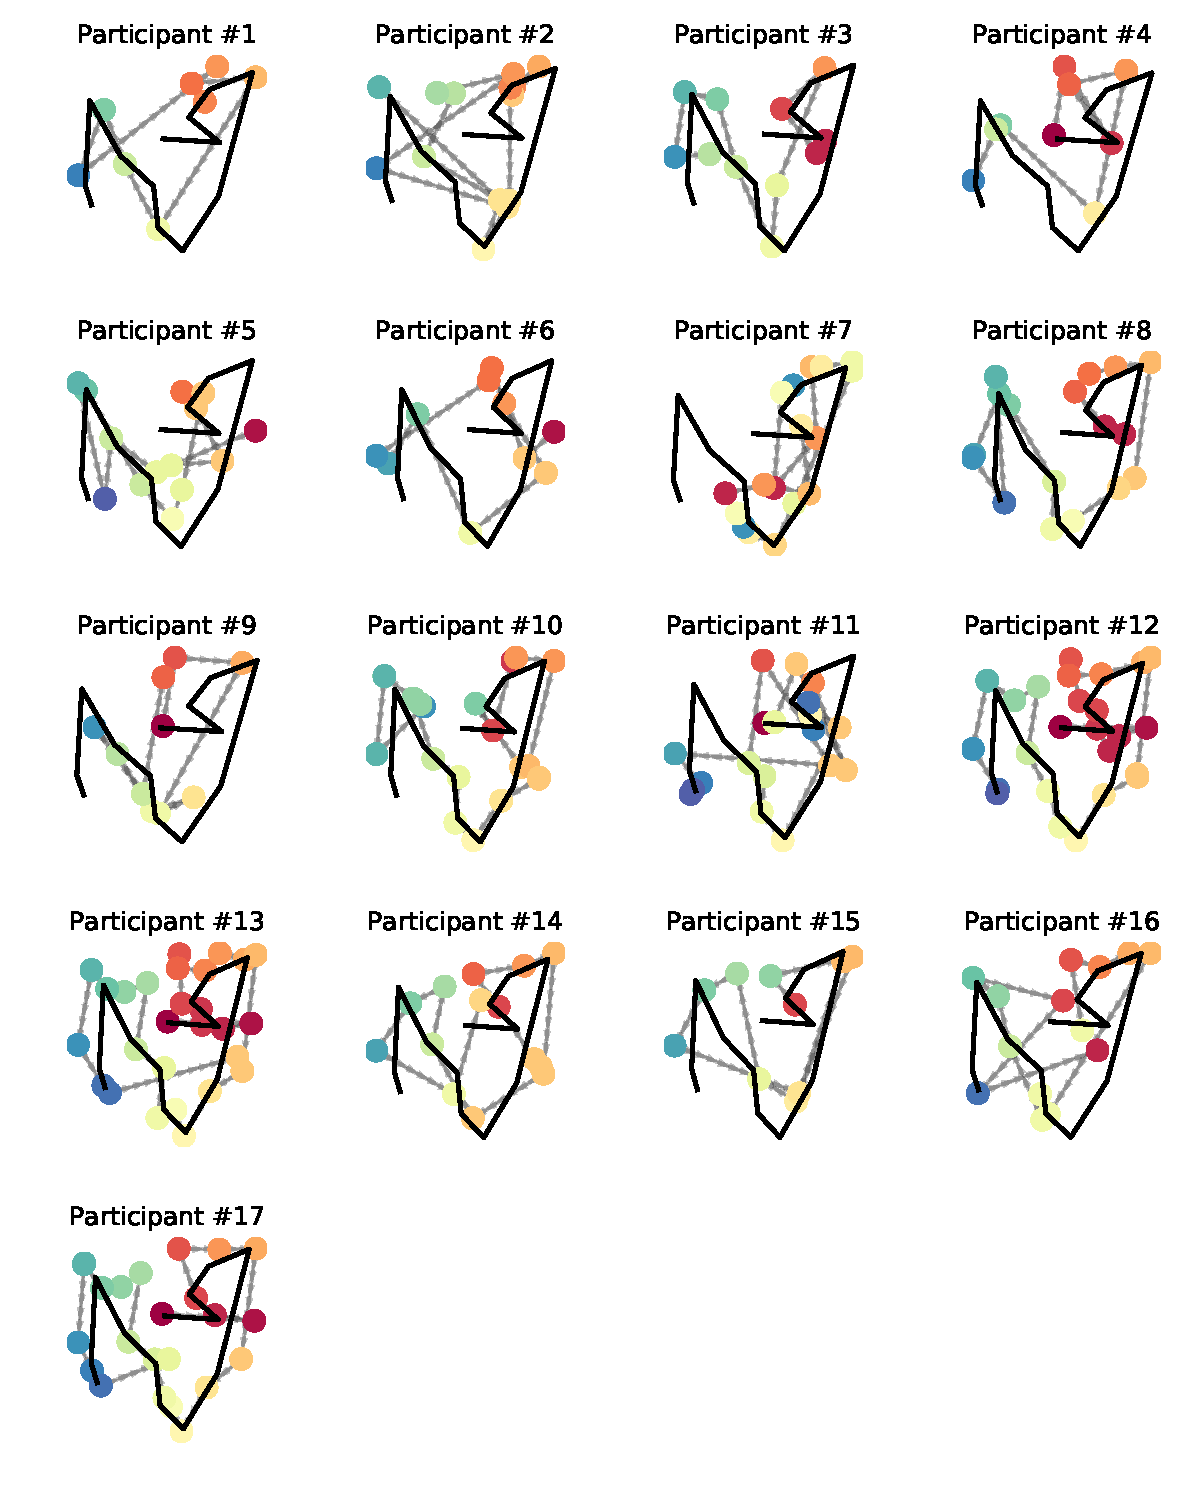
\includegraphics[width=1\textwidth]{figs/supp2_projs.pdf}
\caption{\small \textbf{Individual participant recall event model embeddings.} Each participant's recall event model embedded into a 2D space using the UMAP algorithm. The arrows on the lines connecting the recall events represents the direction of the sequence of recalls.  The color of the dots represent the most likely (i.e. most correlated) video event. The dark black line represents the best fitting line segment model (same for each participant).}
\label{fig:ind_embeddings}
\end{figure}
